\documentclass[12pt]{exam}
\usepackage[utf8]{inputenc}

\usepackage[margin=1in]{geometry}
\usepackage{amsmath,amssymb}
\usepackage{multicol}
\usepackage{mathrsfs}
\usepackage{graphicx}
\usepackage{multicol}
\usepackage[shortlabels]{enumitem}
\usepackage{scrextend}
\usepackage{xcolor}
\usepackage[normalem]{ulem}
\usepackage{optprog}

\newcommand{\class}{SA405, Fall 2022}
\newcommand{\term}{}
\newcommand{\examnum}{Exam 1}
\newcommand{\examdate}{30 September 2022}
\newcommand{\timelimit}{50 Minutes}

\pagestyle{head}
\firstpageheader{}{}{}
\runningheader{\class}{\examnum\ - Page \thepage\ of \numpages}{\examdate}
\runningheadrule

%% Answer box macros
%%\answerbox{alignment}{width}{height}
\newcommand{\answerbox}[3]{%
  \fbox{%
    \begin{minipage}[#1]{#2}
      \hfill\vspace{#3}
    \end{minipage}
  }
}

%%\answerboxfull{alignment}{height}
\newcommand{\answerboxfull}[2]{%
  \answerbox{#1}{6.38in}{#2} 
}

%%\answerboxone{alignment}{height} -- for first-level bullet
\newcommand{\answerboxone}[2]{%
  \answerbox{#1}{6.0in}{#2} 
}

%% special boxes
\newcommand{\wordbox}{\answerbox{c}{1.2in}{.7cm}}
\newcommand{\catbox}{\answerbox{c}{.5in}{.7cm}}
\newcommand{\letterbox}{\answerbox{c}{.7cm}{.7cm}}

 \printanswers
%\noprintanswers
\begin{document}

\noindent
\begin{tabular*}{\textwidth}{l @{\extracolsep{\fill}} r @{\extracolsep{6pt}} r}
\textbf{\class} &&\textbf{\examnum}\\
\textbf{\term} &&\textbf{\examdate}\\
 && \\
 && \\
& \textbf{Name:} & \makebox[2.2in]{\hrulefill}\\\\
%\textbf{Time Limit: \timelimit} &  & \makebox[2in]{\hrulefill}
\end{tabular*}

\noindent
\rule[2ex]{\textwidth}{2pt}

%This exam contains \numpages\ pages (including this cover page) and \numquestions\ questions.\\
%Total of points is \numpoints.

\begin{itemize}
%\item You may pull the pages apart and then staple them together at the end.  I prefer not to see your name when I am grading, so only write your name on the first page (unless submitting pages unstapled).

\item %No books, notes, or any other outside help % or calculators
% that do symbolic manipulation (such as TI-89 or TI-92) 
 %allowed. %
 {\bf One sided} 8.5 by 11 inch formula/note sheet is allowed.

%\item You may use your calculator on this test.

\item Show work clearly and neatly.  

\item Define all notation used.
%\item If you need more space than is provided, use the back of the previous page. 

\item Please read each question carefully.
If you are not sure what a question is
asking, ask for clarification.

\item If you start over on a problem, please CLEARLY indicate what your final
  answer is, along with its accompanying work.

%\item All formulations must have descriptions of any indices, parameters, and decision variables used. All constraints must be described. 
\end{itemize}

\bigskip
\begin{center}
Grade Table (for teacher use only)\\
\addpoints
\gradetable[v][questions]
\end{center}

\noindent
\rule[2ex]{\textwidth}{2pt}

% I think this is a requirement now
\emph{Please write the following statement and sign it.}\\
The Naval Service I am a part of is bound by honor
and integrity. I will not compromise our values by
giving or receiving unauthorized help on this exam.

\newpage %%%%%%%

\newpage

\begin{questions}

% Adjust points as you'd like, we can make it add up to 100 when the whole thing is done

\question Gandalf has decided to transport the 19 rings of power from various parts of Middle-Earth to the Southlands in order to combat evil Sauron's power. Five of the rings originate in Numenor, ten rings originate in Lothloren, and the remaining four rings originate in Rivendell. To transport the rings from these cities to the Southlands, they can be transported through the following cities/towns: Mithlond, the Shire, and Helm's Deep. To send rings through various cities is quite risky. The following table depicts the level of risk for transporting a single ring from one city to another:
\begin{center}
\begin{tabular}{c|cccc}
 &  & \textbf{To} &  \\
\textbf{From} & (M) Mithlond& (T) The Shire &  (H) Helm's Deep & (S) The Southlands\\ \hline
(N) Numenor & 5 & 3 & 4 & --  \\
(L) Lothloren  & 7 & 2 & 5& --  \\
(R) Rivendell & 2 & 6 & 7& --  \\
(M) Mithlond & -- & -- & -- & 17 \\
(T) The Shire & -- & -- &  -- & 12 \\
(H) Helm's Deep & -- & -- & -- & 18
\end{tabular}
\end{center}

Assuming that you cannot transport the rings directly from their origination points, Gandalf wants to minimize the total risk of moving the 19 rings from the three cities all to the Southlands.  All 19 rings must be transported through Mithlond, The Shire, or Helm's Deep.

We define the following variables:

Let $x_{i,j}$ be the number of rings shipped from city $i$ to city $j$ (that is $x_{N,M}$, $x_{N,T}$,$\hdots$, $x_{H,S}$)


\begin{parts}
    \part[8] In the \emph{abbreviated} concrete form, write the objective function set forth from Gandalf.
\begin{solution}
\[
\text{min } 5 x_{N,M} + 3 x_{N,T} + \cdots + 18 x_{H,S}
\]
\end{solution}
    
    \vfill
    \part[6] In the concrete from, write the flow-balance constraint for the island city of Numenor. 
\begin{solution}
\[
5 = x _{N,M} + x_{N,T} + x_{N,H}
\]
\end{solution}
    
    \vfill \newpage
    \part[6] In the concrete from, write the flow-balance constraint for the castle of Helm's Deep.
\begin{solution}
\[
x_{N,H} + x_{L,H} + x_{R,H} = x_{H,S}
\]
\end{solution}    
    
    \vfill
    \part[6] In the concrete from, write the flow-balance constraint for The Southlands.

\begin{solution}
\[
x_{M,S} + x_{T,S} + x_{H,S} = 19
\]
\end{solution}
    
    \vfill
    \part[6] Finally, write constraint(s) to ensure that no more than 9 rings can travel through each of the three relay towns (Mithlond, The Shire, and Helm's Deep).

\begin{solution}
There's two solutions, either restrict flow in to the cities or flow out of the cities. I'll do the flow in below:
\begin{optprog*}
& x_{N,M} + x_{L,M} + x_{R,M} & \leq & 9 \\
& x_{N,T} + x_{L,T} + x_{R,T} & \leq & 9 \\
& x_{N,H} + x_{L,H} + x_{R,H} & \leq & 9
\end{optprog*}
\end{solution}
    
    \vfill
\end{parts}
\newpage
\question Last Spring, Professor Alameda decided to leave USNA to open up his own muffin bakery. Against all odds, business has been great! He is considering opening up $2$ new bakeries that would serve $3$ stores in the nearby area. The following table shows the cost of opening each bakery (in thousands), the amount of muffins truckloads each store demands, and the transportation cost (in thousands) per truckload of muffins from each bakery to each store. Assume each bakery can supply $44$ truckloads of muffins. Professor Alameda needs your help to decide which bakeries to open in order to minimize his costs! 

\begin{center}
\begin{tabular}{c|c|ccc}
& Bakery & \multicolumn{3}{c}{Transport Costs} \\
& Cost & Store 1 & Store 2 & Store 3 \\
\hline
Bakery 1 & 200 & 6 & 5 & 9   \\
Bakery 2 & 400 & 4 & 3 & 5  \\

\hline
Demand & --- & 11 & 18 & 15 
\end{tabular}
\end{center}

\begin{parts}
    \part[10] Ignoring the bakery opening cost, write out a concrete model that minimizes the total transportation cost (make sure to define all variables for full credit).
    
    \begin{solution}
\textbf{Decision Variables:} Let $x_{1,1}$ be the flow from bakery 1 to store 1, $x_{1,2}$ be the flow from bakery 1 to store 2, etc.

\textbf{Objective}
\[
\text{min } 6 x_{1,1} + 5 x_{1,2} + \cdots + 5 x_{2,3}
\]    

\textbf{Constraints}
\begin{optprog*}
& x_{1,1} + x_{1,2} + x_{1,3} & \leq & 44 & \text{(supply 1)} \\
& x_{2,1} + x_{2,2} + x_{2,3} & \leq & 44 & \text{(supply 2)} \\
& x_{1,1} + x_{2,1} & = & 11 & \text{(demand 1)} \\
& x_{1,2} + x_{2,2} & = & 18 & \text{(demand 2)} \\
& x_{1,3} + x_{2,3} & = & 15 & \text{(demand 3)} \\
& x_{1,1}, \ldots, x_{2,3} & \geq & 0 & \text{(non-negativity)}
\end{optprog*}  
 
    \end{solution}
    
    
    \part[10] Modify your formulation from part (a) to incorporate the bakery opening costs and any constraints associated with opening the bakeries. Be sure to clearly define any new variable(s) used.

\begin{solution}
Define two new binary variables: $z_1 = 1$ if bakery 1 is open and $z_2 = 1$ if bakery 2 is open.

Modify objective function to be:
\[
\text{min } 6 x_{1,1} + 5 x_{1,2} + \cdots + 5 x_{2,3} + 200 z_1 + 400 z_2
\]

Add forcing constraints. One way to do this are the following two constraints:
\begin{optprog*}
& x_{1,1} + x_{1,2} + x_{1,3} & \leq & 44 z_1 \\
& x_{2,1} + x_{2,2} + x_{2,3} & \leq & 44 z_2 
\end{optprog*}

Also add binary constraints:
\[
z_1, z_2 \in \{0,1\}
\]

\end{solution}    
    
    %Modify the objective function in the model from part (a) to incorporate the bakery opening cost, and write out the necessary fixed charge constraints. (You might need a new variable)
    
    \newpage
    \part[15] Parameterize your completed model. Be sure to clearly define all sets, variables, and parameters for full credit.
\end{parts}

\begin{solution}
\textbf{Sets}

Let $B$ be the set of bakeries\\
Let $S$ be the set of stores

\textbf{Parameters}

Let $c_{i,j}$ be the cost of shipping from bakery $i$ to store $j$ for all $i \in B$ and $j \in S$ \\
Let $s_i$ be the supply of bakery $i$ for all $i \in B$ \\
Let $d_j$ be the demand of store $j$ for all $j \in S$ \\
Let $f_i$ be the fixed cost of opening store $i$ for all $i \in B$

\textbf{Variables}

Let $x_{i,j}$ be the number of muffins sent from bakery $i$ to store $j$ for all $i \in B$ and $j \in S$\\
Let $z_i = 1$ if bakery $i$ is open and $0$ otherwise for all $i \in B$

\textbf{Objective}

\[
\text{min } \sum_{i \in B} \sum_{j \in S} c_{i,j} x_{i,j} + \sum_{i \in B} f_i z_i
\]

\textbf{Constraints}

\begin{optprog*}
& \sum_{j \in S} x_{i,j} & \leq & s_i z_i & \text{for $i \in B$} & \text{(supply and forcing)} \\
& \sum_{i \in B} x_{i,j} & = & d_j & \text{for $j \in S$} & \text{(demand)} \\
& x_{i,j} & \geq & 0 & \text{for $i \in B$ and $j \in S$} & \text{(non-negative)} \\
& z_i & \in & \{0,1\} & \text{for $i \in B$} & \text{(binary)}
\end{optprog*}

\end{solution}

\newpage

% This is set covering with either/or and if/then constraints
\question Consider the following network with nodes $N$ and edges $E$:

\begin{center}
    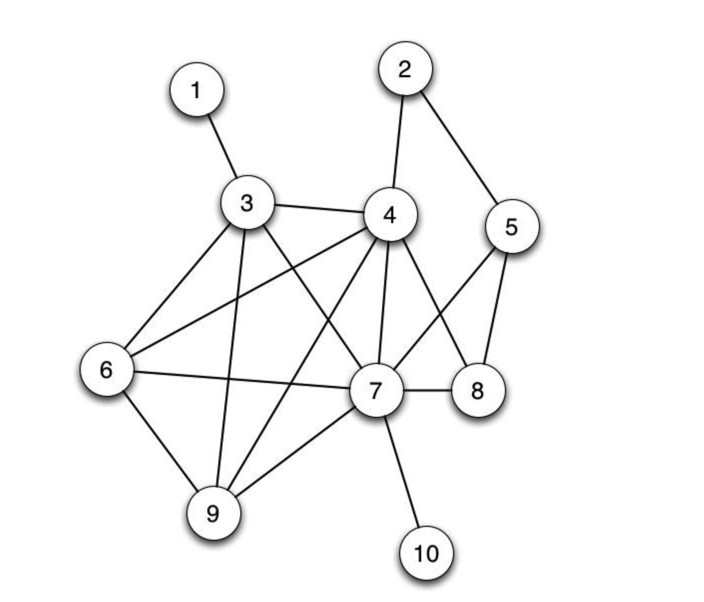
\includegraphics[width=0.8\textwidth]{network10nodes.jpeg}
\end{center}

A \textbf{node covering} is a collection of nodes in the graph such that every edge in $E$ has at least one endpoint in the collection. For example, for edge $(1,3)$ selecting either node $1$ or node $3$ covers this edge. The goal is to minimize the number of nodes selected for the covering. 

Let 
\[
x_i = \begin{cases} 1 & \text{if node $i$ is selected for the covering} \\
                    0 & \text{if node $i$ is not selected for the covering}
\end{cases}
\] for all $i \in N$.

\begin{parts}
    \part[5] Write a concrete objective function which could be used to select a covering consisting of the fewest number of nodes.

    \begin{solution}
        \[
            \text{min } x_1 + x_2 + \cdots + x_{10}
        \]
    \end{solution}

\newpage
    \part[6] Write two constraints, one that would ensure edge $(2,5)$ is covered and another which would ensure edge $(6,7)$ is covered.

\vfill
    
    \begin{solution}
        \[
            x_2 + x_5 \geq 1
        \]
        \[
            x_6 + x_7 \geq 1
        \]
    \end{solution}

    \part[5] Parameterize your constraints from part (b) such that we have one parameterized constraint that covers all edges in the network.
    \begin{solution}
    \[
        x_i + x_j \geq 1 \text{ for all $(i,j) \in E$}
    \]
    \end{solution}
\vfill    
    \part Suppose that there is a cost associated with placing a sensor at each node. Two companies offer bids for the sensors. The first company offers a flat rate of \$100 for each sensor but at least 5 sensors much be purchased. The second company offers a rate of \$150 for each sensor with no minimum number requirement. There's a total budger of \$600. You write the following constraints:
    \begin{optprog*}
    (A) & 100 x_1 + 100 x_2 + \cdots + 100 x_{10} & \leq & 600 \\
    (B) & x_1 + x_2 + \cdots + x_{10} & \geq & 5 \\
    (C) & 150 x_1 + 150 x_2 + \cdots + 150 x_{10} & \leq & 600
    \end{optprog*}

You define a binary variable $z$. $z = 1$ if sensors are purchased from company 1 and $z = 0$ if sensors are purchased from company 2. Modify these constraints such that:
    \begin{subparts}
    \subpart[6] Constraints (A) and (B) are enforced if $z = 1$ and relaxed if $z = 0$. 

    \begin{solution}
    \begin{optprog*}
    (A) & 100 x_1 + 100 x_2 + \cdots + 100 x_{10} & \leq & 600 + M (1-z) \\
    (B) & x_1 + x_2 + \cdots + x_{10} & \geq & 5  - M(1-z)
    \end{optprog*}
        
    \end{solution}
    \vfill
    \subpart[4] Constraint (C) is relaxed if $z = 1$ and enforced if $z = 0$.

    \begin{solution}
    \[
    150 x_1 + 150 x_2 + \cdots + 150 x_{10} \leq 600 + M z
    \]
    \end{solution}
    
    \end{subparts}
\vfill

\newpage
    \part[3] Suppose that if node $3$ is not selected than node $4$ must be selected. Write a constraint to enforce this requirement.
        \begin{solution}
            \[
            1-x_3 \leq x_4
            \]
        \end{solution}      
        \vfill
    \part[4] Likewise, suppose that if node $6$ is selected then node $3$ must also be selected and node $4$ can not be selected. Write constraint(s) to enforce this requirement.
    \begin{solution}
        \[
        2 x_6 \leq x_3 + (1-x_4)
        \]
    \end{solution}      
\end{parts}
\vfill


\end{questions}
\end{document}
